\subsection{Alessio Minniti}
\subsubsection{Turnation Manager}
\begin{figure}[H]
    \centering
    \makebox[1.0\textwidth]{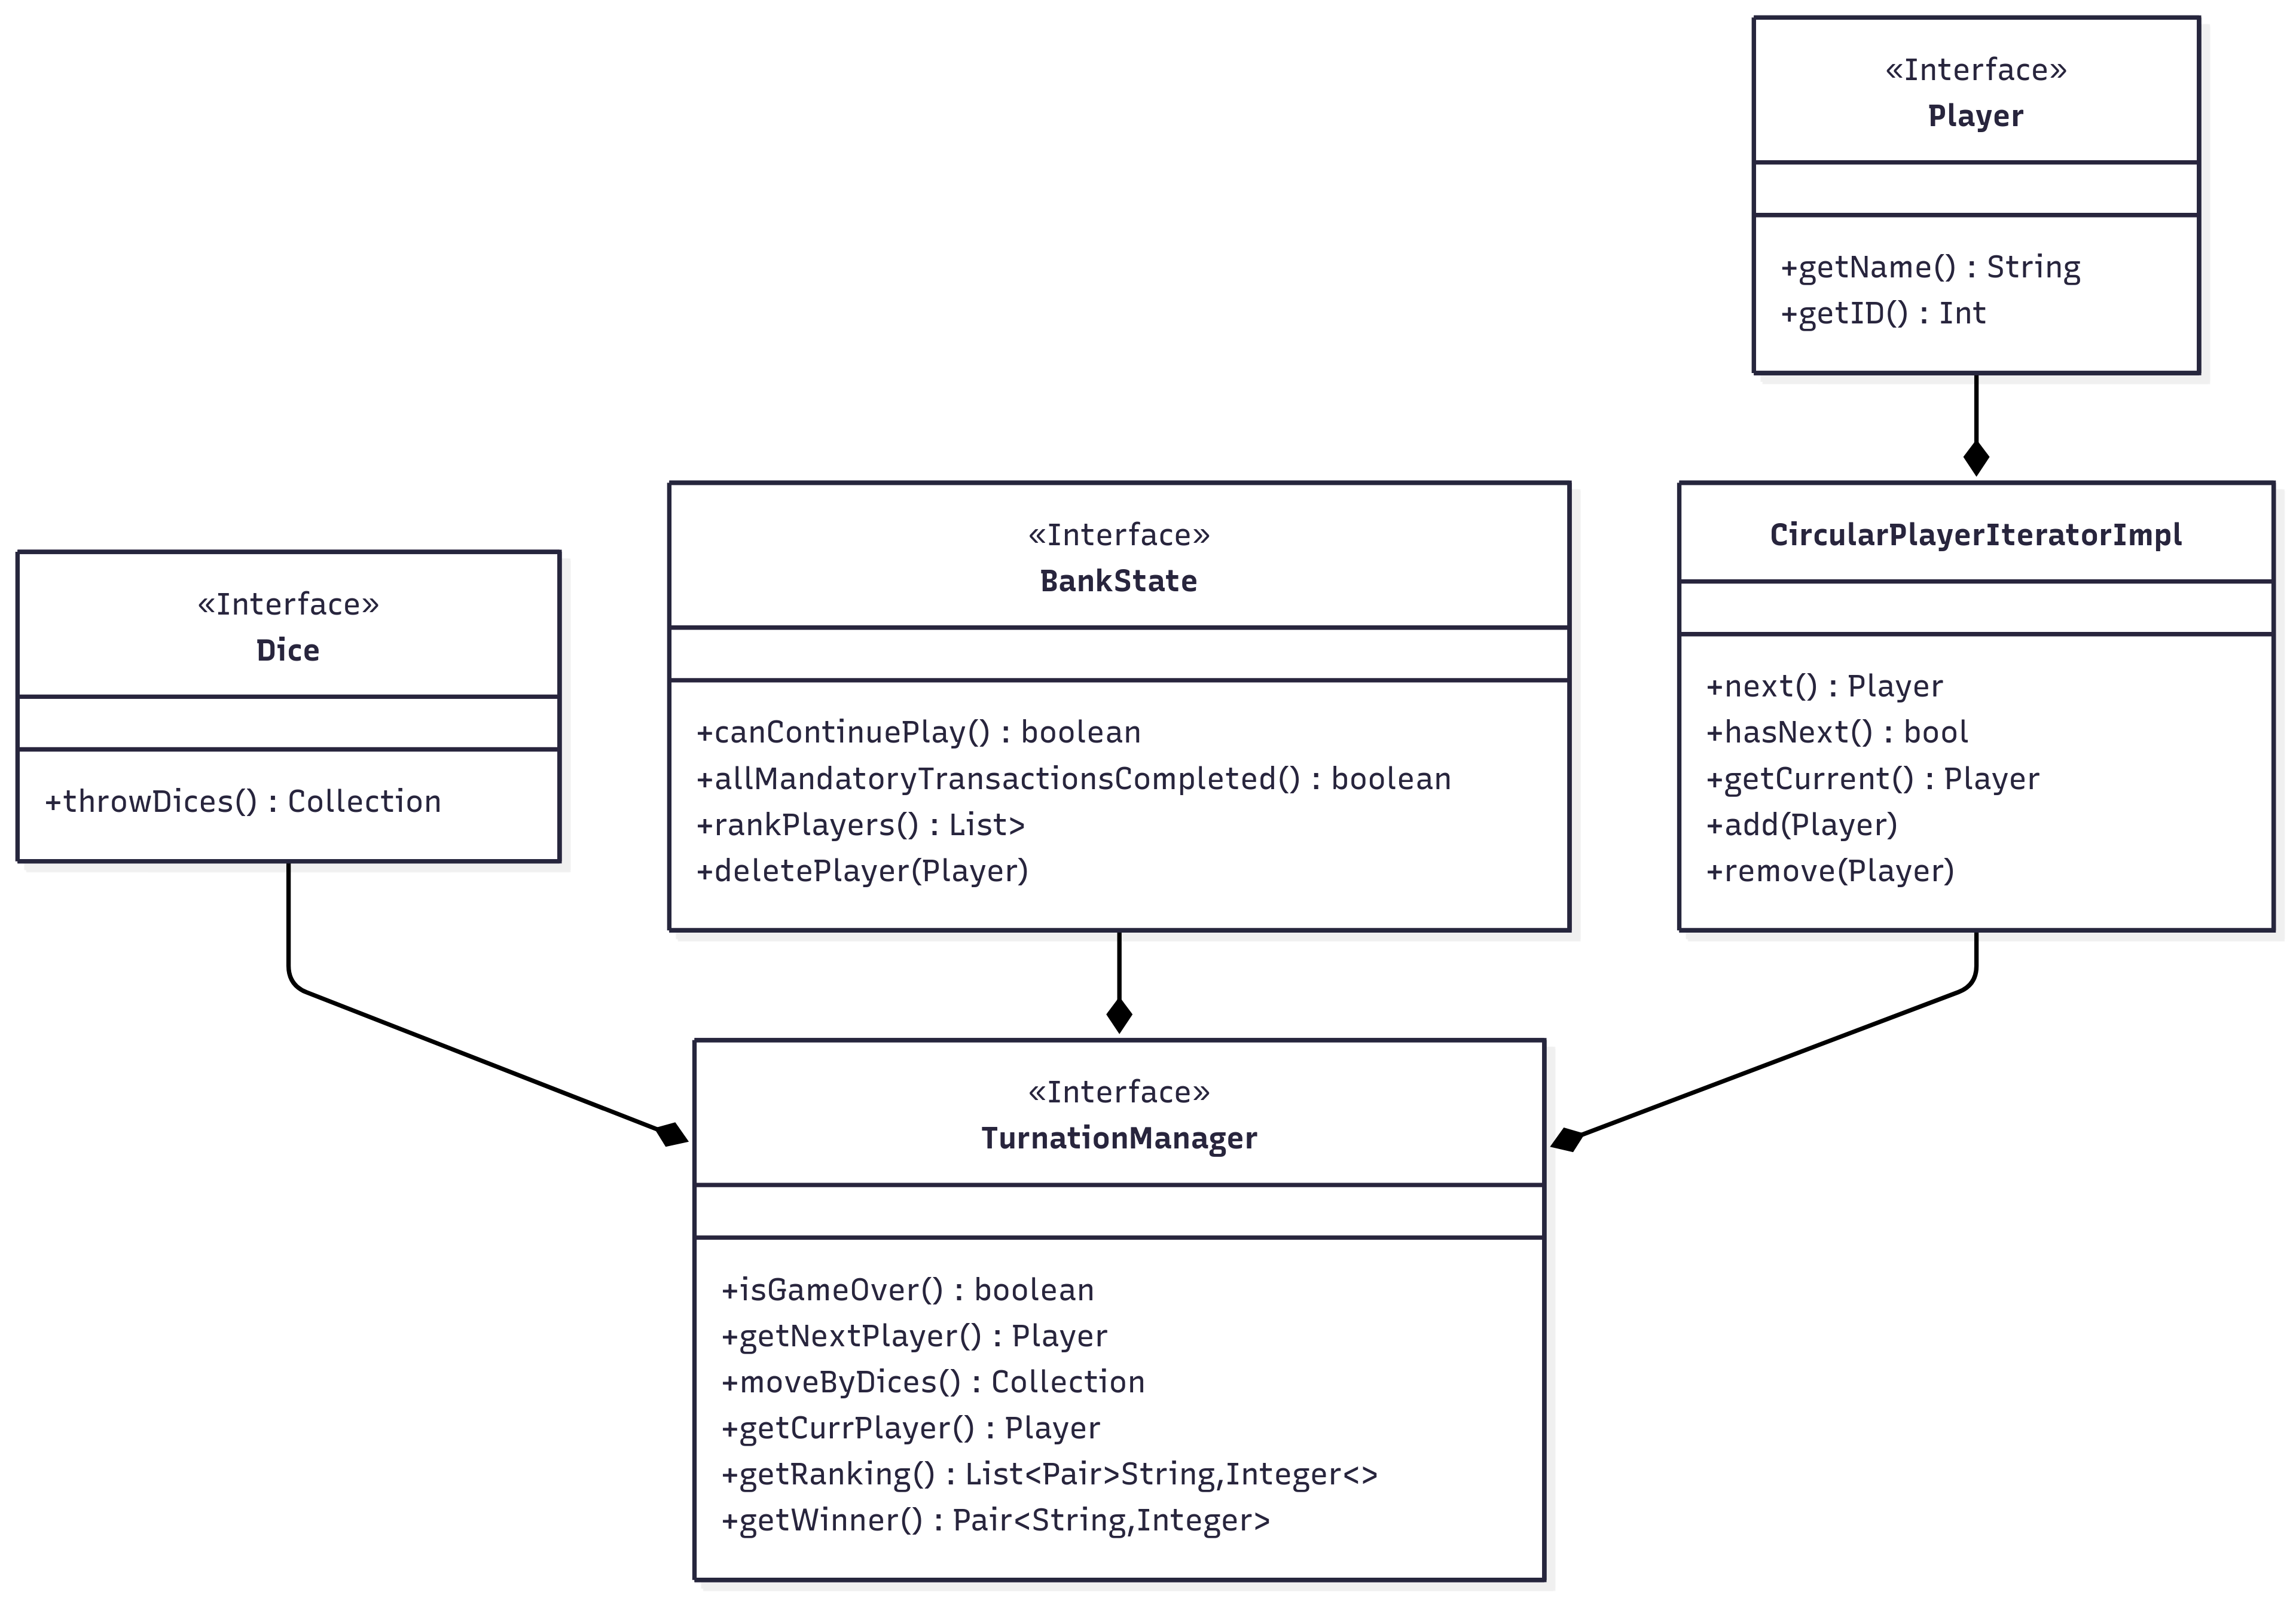
\includegraphics[width=1\textwidth]{img/minniti/turnationManager.png}}	
    \caption{Schema UML della struttura del Turnation Manager, il Turnation Manager gestisce una lista di player che viene iterata ciclicamente, 
    il Dice che permette il lancio dei dadi e Il BankState che permette la comunicazione con la Bank }
	\label{img:Turnation}
\end{figure}

Il \textbf{Turnation Manager} ha il compito di gestire lo stato dei \textbf{player} e i loro turni, 
infatti permette e controlla il lancio dei dadi, la terminazione del turno, gli stati di prison e park del player e lo stato del ranking dei players.\newline

Per farlo il Turnation Manager usa una \textbf{lista circolare di player} usata per ricavarne il \textbf{current player} per capire chi deve eseguire il turno e
quando la lista arriva all'ultimo player ricomincia dall'inizio senza però contenere più i player che sono morti nel turno precedente.\newline
Inoltre ha un oggetto \textbf{Dice} che all'interno possiede una serie di random in modo che si possano lanciare 
un numero a piacere di dadi da un numero di facce a piacere che viene definito alla creazione. Con questa realizzazione è quindi possibile avere future implementazioni del gioco
dove si usano quanti dadi si vuole e con quante facce si vuole.\newline
Infine utilizza il \textbf{BankState} per controllare che un player abbia fatto tutte le azioni di compravendita obbligatorie prima di terminare il turno.
Inoltre bankState viene utilizzato dal Turnation Manager anche per determinare il ranking finale e il vincitore alla fine del gioco.

\subsubsection{Circular Player Iterator}
\begin{figure}[H]
    \centering
    \makebox[0.5\textwidth]{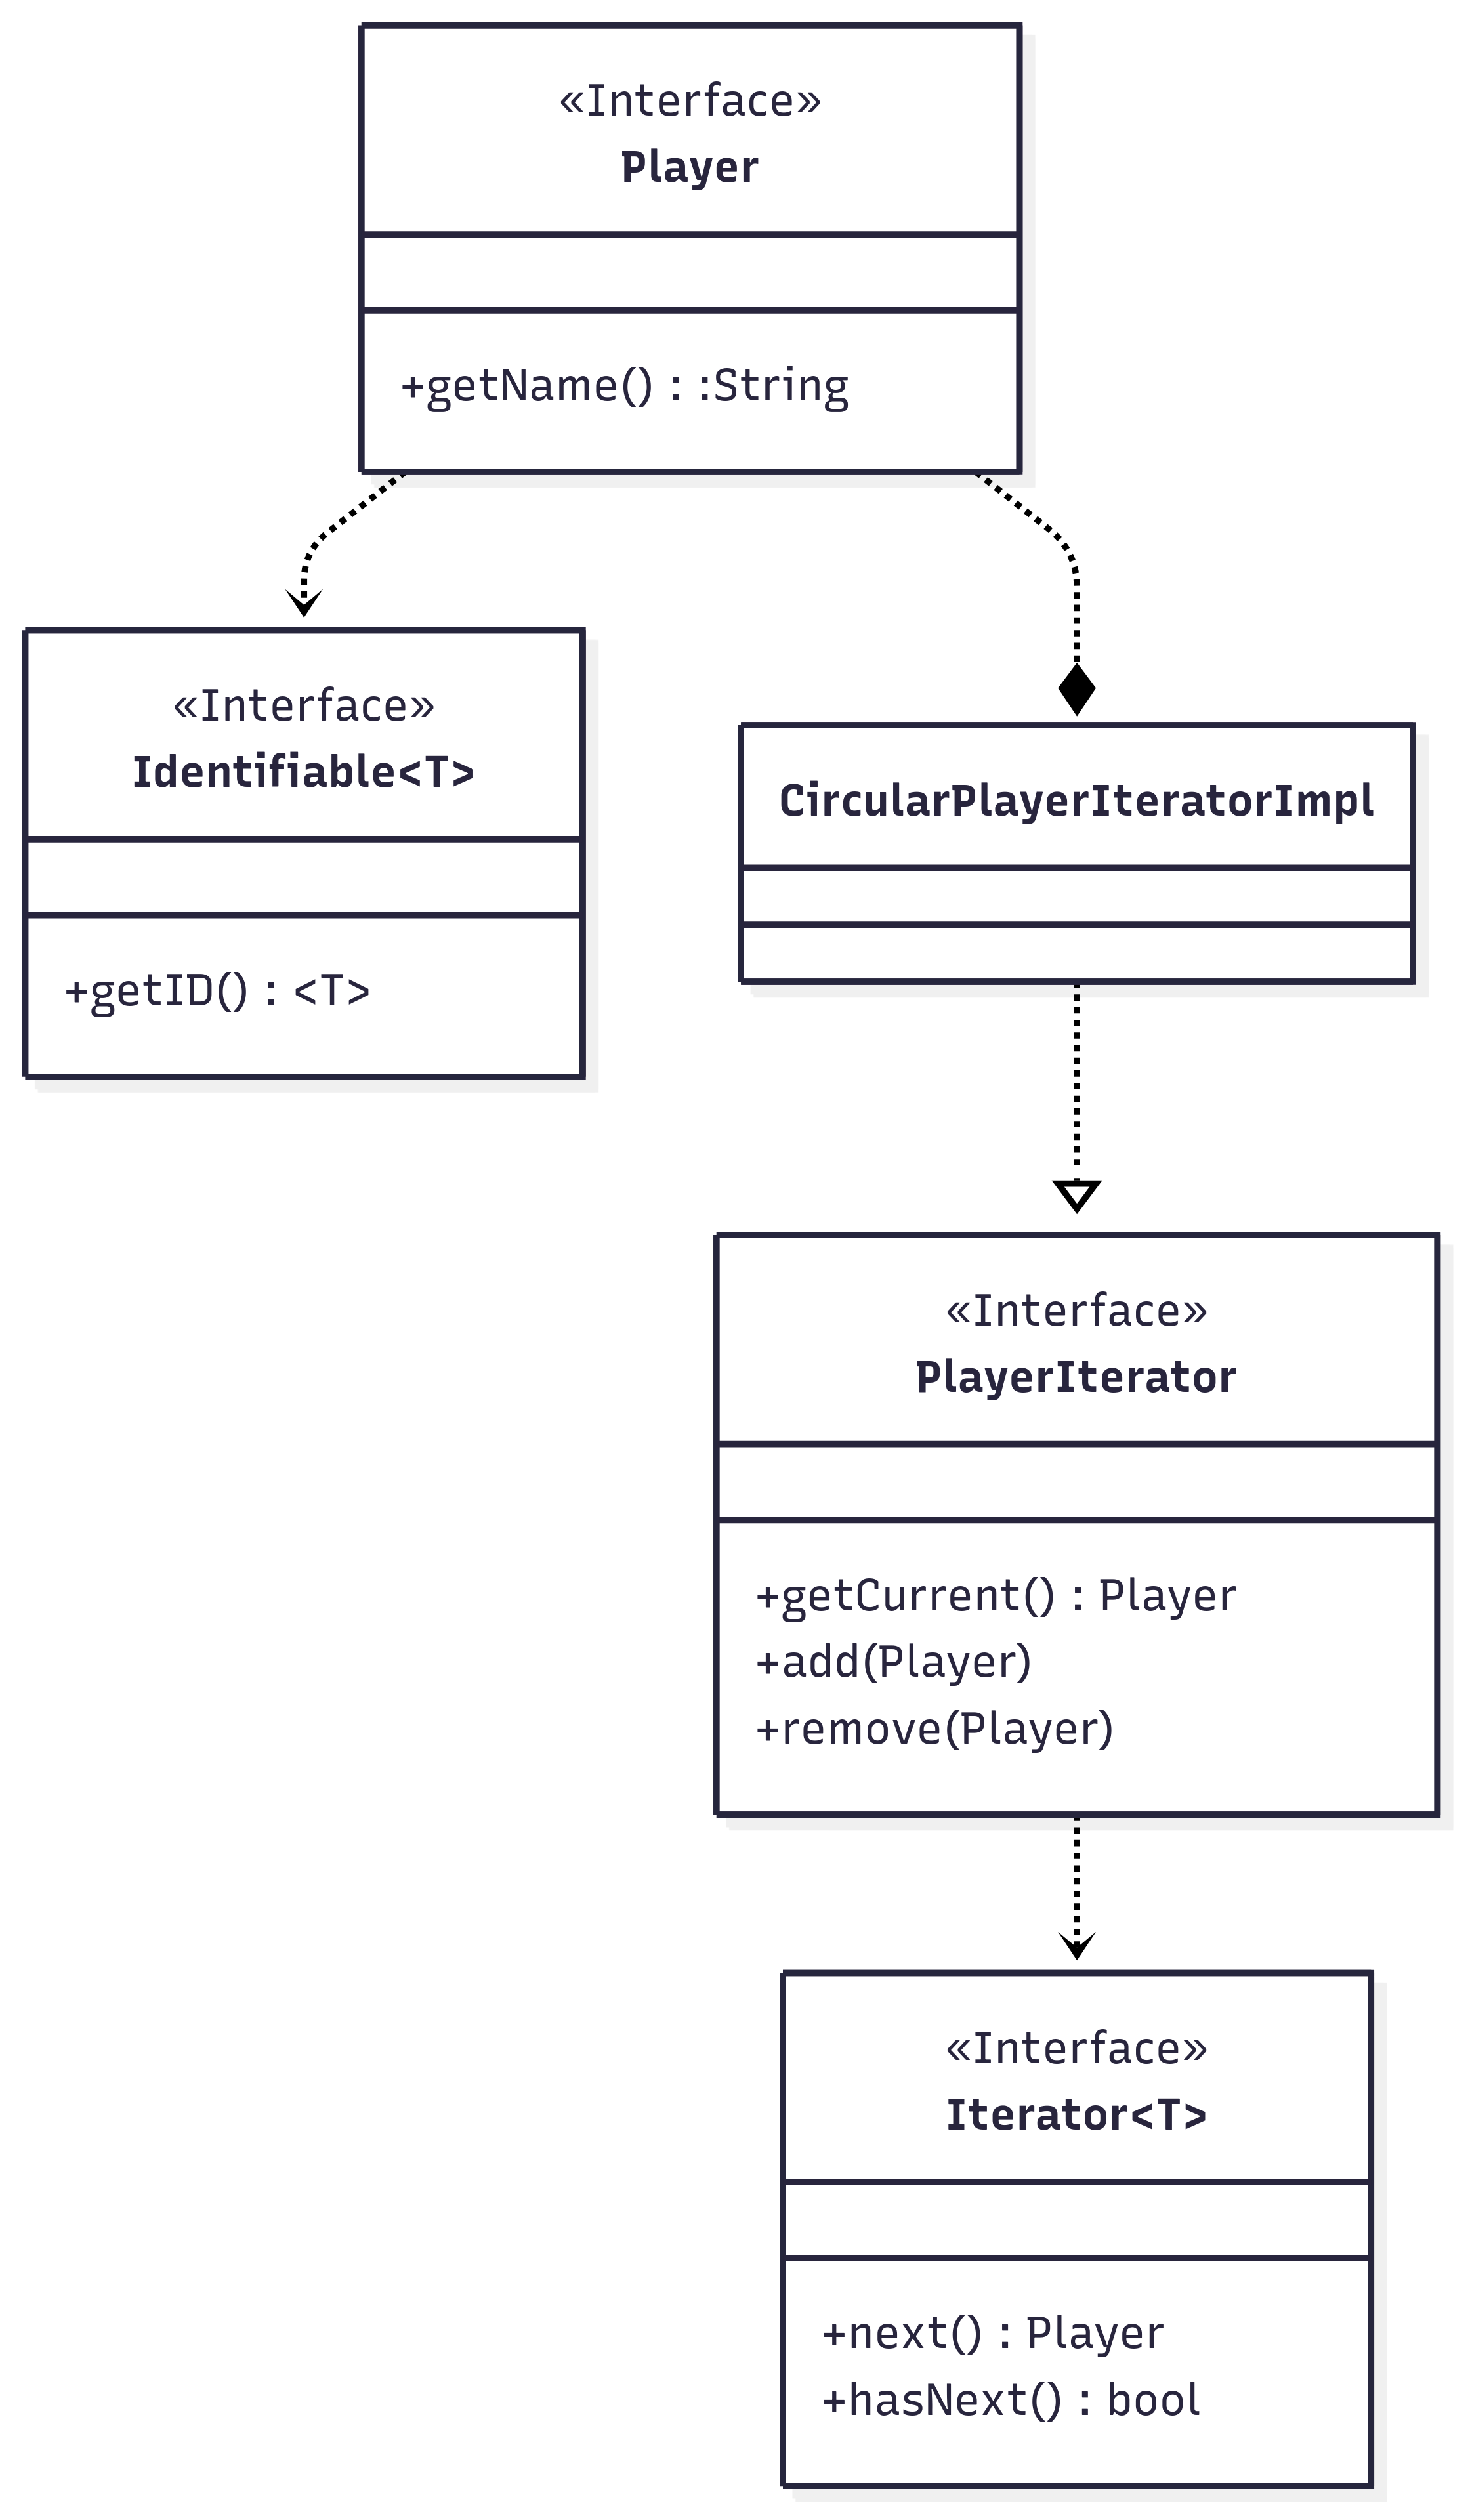
\includegraphics[width=0.5\textwidth]{img/minniti/iterator.png}}	
    \caption{Schema UML che definisce il funzionamento della struttura dati circolare dei player, Il Circular Player Iterator è un'implementazione ciclica del Player Iterator,
    un' estensione di iterator pensata per gestire i player}
	\label{img:Iterator}
\end{figure}

PROBLEMA:
Il Turnation Manager per gestire i turni dei player ha bisogno di una struttura dati che passa sempre il prossimo player in modo ciclico, 
quindi una volta che arriva all'ultimo player deve ricominciare ad assegnare i turni dal primo player, tuttavia di base non c'è una lista circolare 
e cercando tra le librerie esterne non ne ho trovata una che ne forniva una adeguata.\newline

SOLUZIONE:
Per risolvere questo problema quindi ho utilizzato il pattern \textbf{iterator}, andando a creare un' interfaccia \textbf{PlayerIterator} che estende iterator 
e serve a definire le azioni cardine del circular player iterator che oltre ad avere i metodi di un iteratore normale possiede anche funzioni aggiuntive per gestire la lista di player,
l'implementazione del player iterator \textbf{Circular Player Iterator} wrappa la lista di player e itera la lista ritornando sempre il prossimo player 
che deve svolgere il turno in maniera ciclica, quindi quando vede che è arrivato all'ultimo player ricomincia ad iterare la lista dall'inizio.\newline

\subsubsection{Board}
\begin{figure}[H]
    \centering
    \makebox[1.0\textwidth]{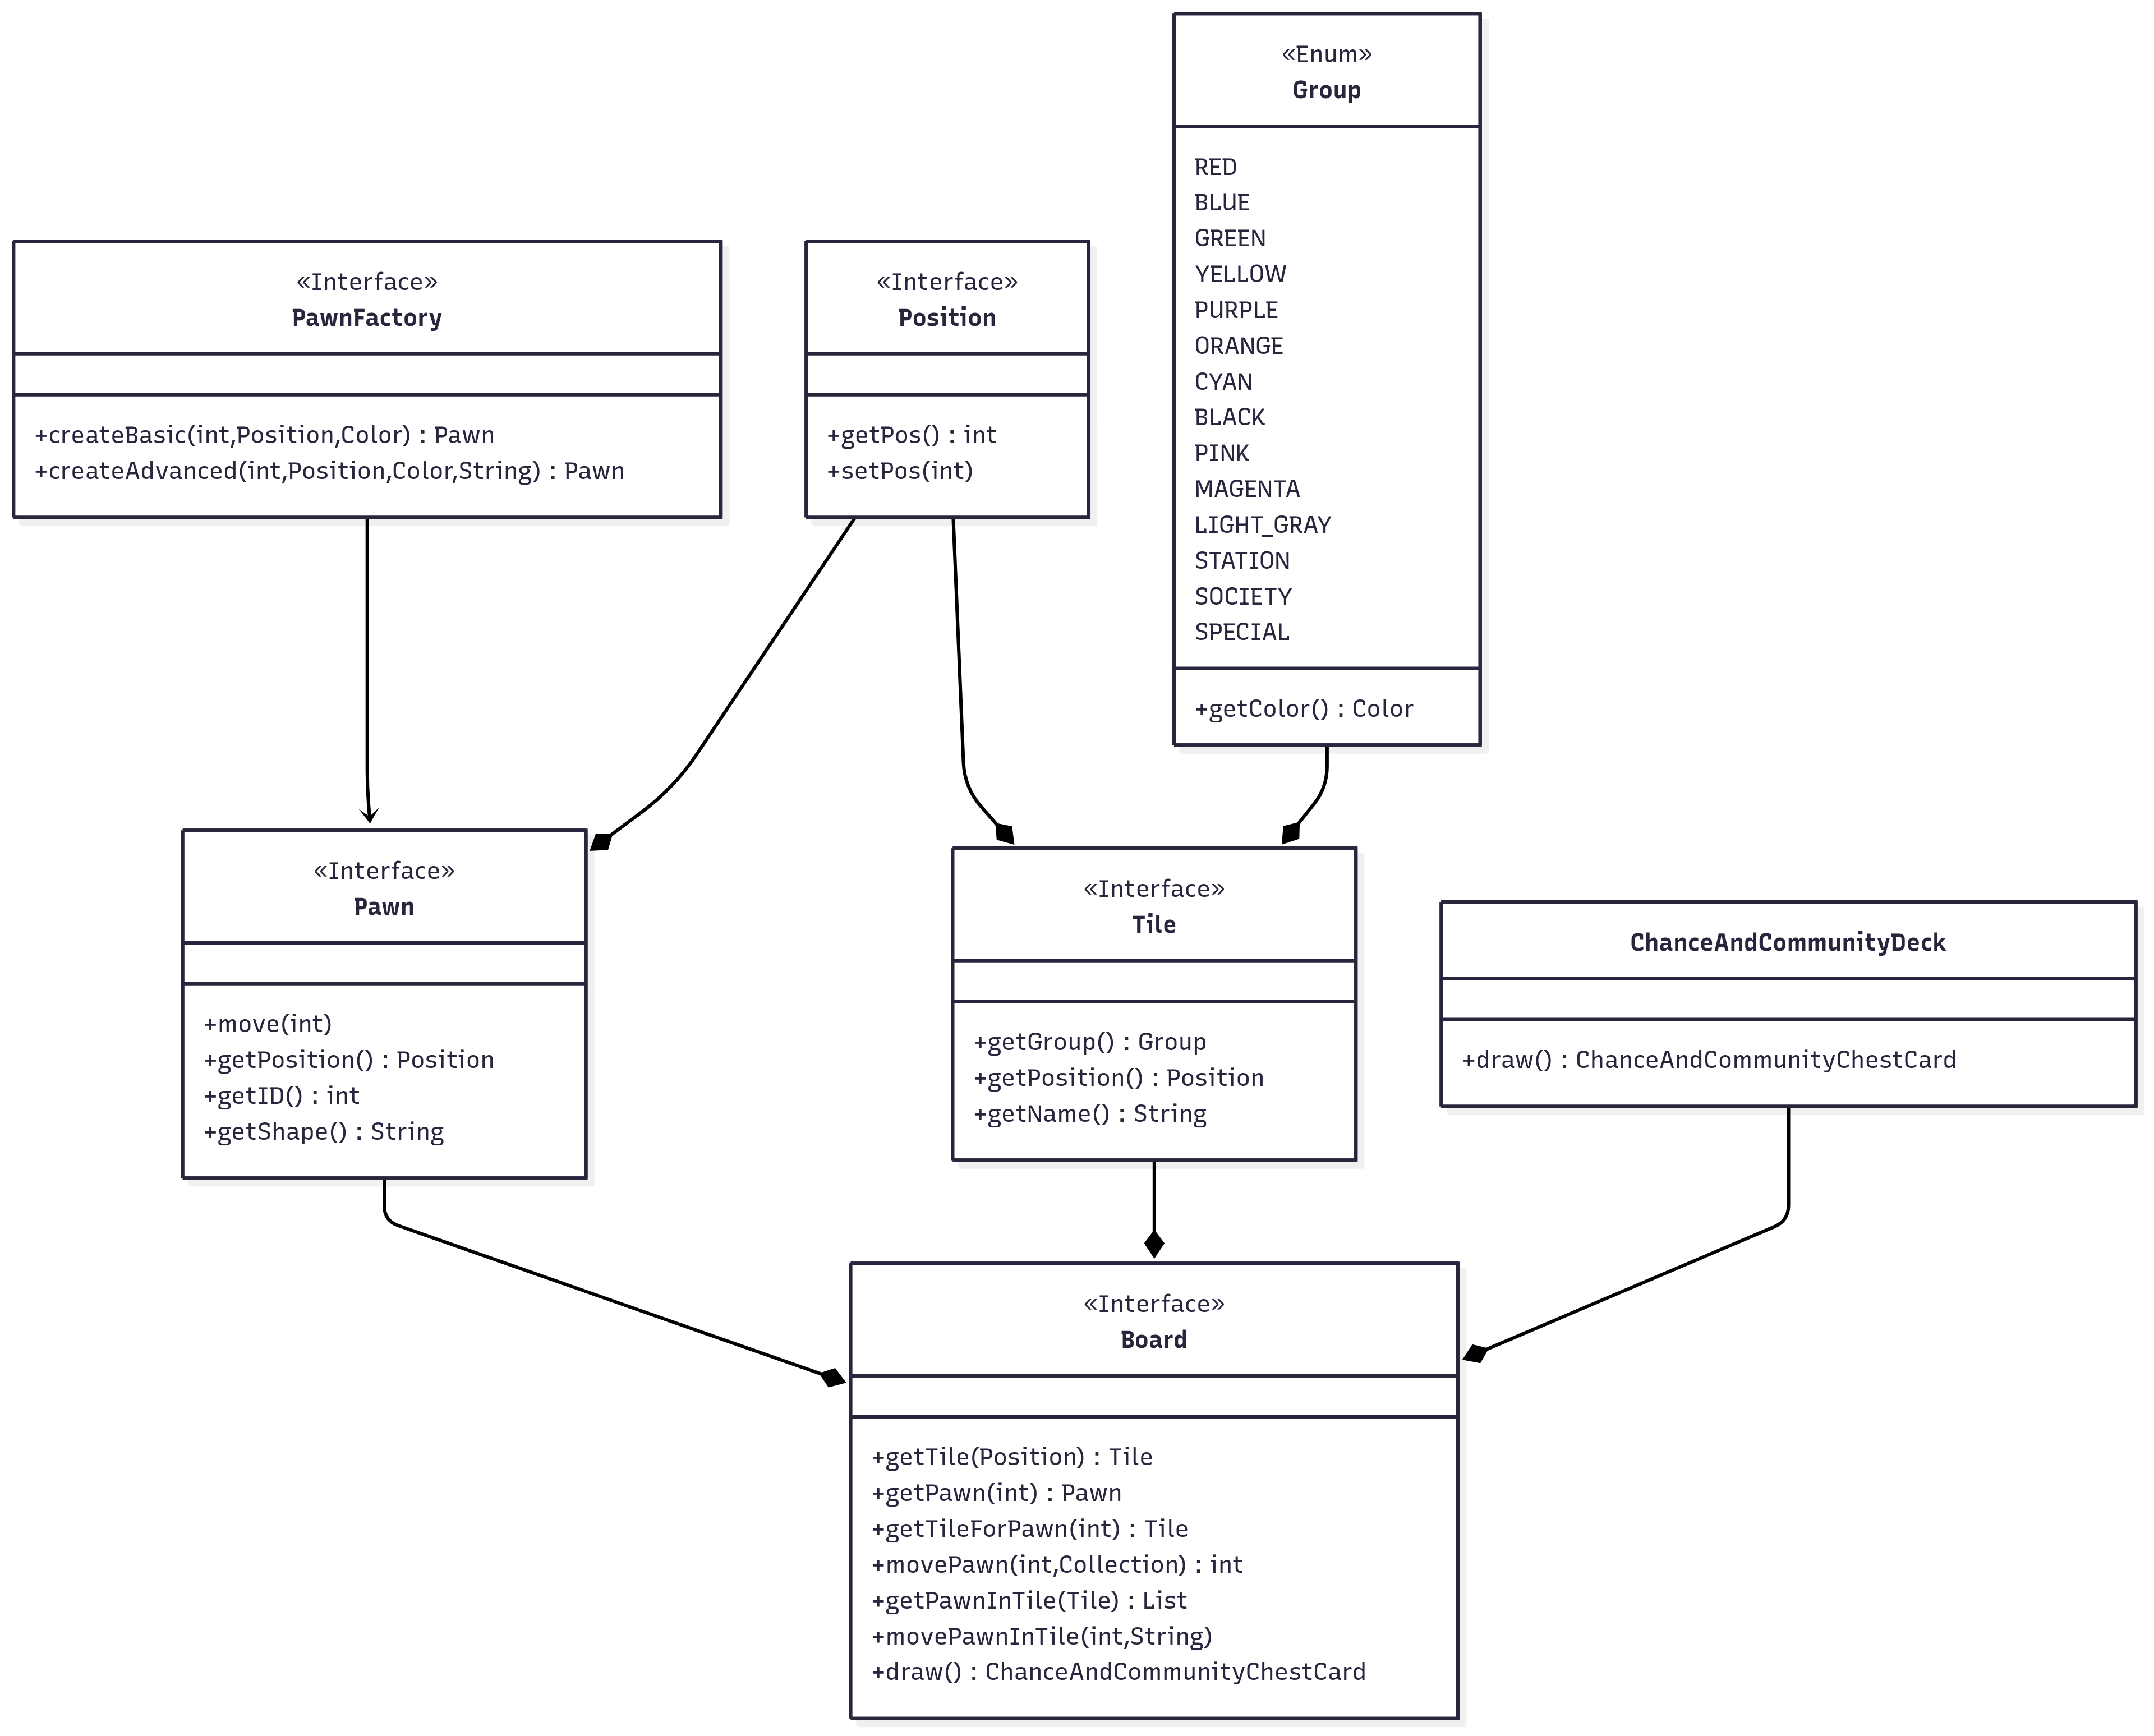
\includegraphics[width=1.3\textwidth]{img/minniti/board.png}}	
    \caption{Schema UML che definisce il funzionamento di Board, esso gestisce tutte le azioni da svolgere sulle pawns, sulle tiles e sul deck}
	\label{img:Board}
\end{figure}
La \textbf{Board} ha il compito di gestire le \textbf{Tiles} e le \textbf{Pawns} con le loro posizioni, e il \textbf{deck} delle carte chance e community, 
gestisce il movimento delle pawns ricavato dal lancio del dado che gli viene passato e tiene traccia di tutti i loro cambiamenti di posizioni,
tiene traccia di tutte le posizioni delle caselle ed inoltre gestisce anche la creazione e rimozione delle case e alberghi nelle proprietà.\newline

PROBLEMA:
Quando la board deve restituire le pawns, essendo che non deve permettere il loro cambio di posizione al di fuori della board, 
essa deve restituire oggetti immutabili per prevenire eventuali modifiche. 
Per risolverlo si potrebbe richiamare sempre il costruttore delle pawn ma non mi sembrava il metodo più efficiente \newline

SOLUZIONE:
Quindi Per facilitare tale operazione ho usato il pattern \textbf{factory method}, andando a creare l'interfaccia \textbf{PawnFactory} 
che con la sua relativa implementazione possiede i metodi \textbf{createBasic} che permette di creare la pawn normale senza shape
e \textbf{createAdvanced} che permette di creare la pawn con la shape in caso in cui in future versioni del gioco si voglia far scegliere la forma della propria pedina al giocatore. 
Usando quindi una factory evito di dover richiamare sempre il costruttore per ritornare copie immutabili.\newline

\subsubsection{Tiles e Property}
\begin{figure}[H]
    \centering
    \makebox[0.5\textwidth]{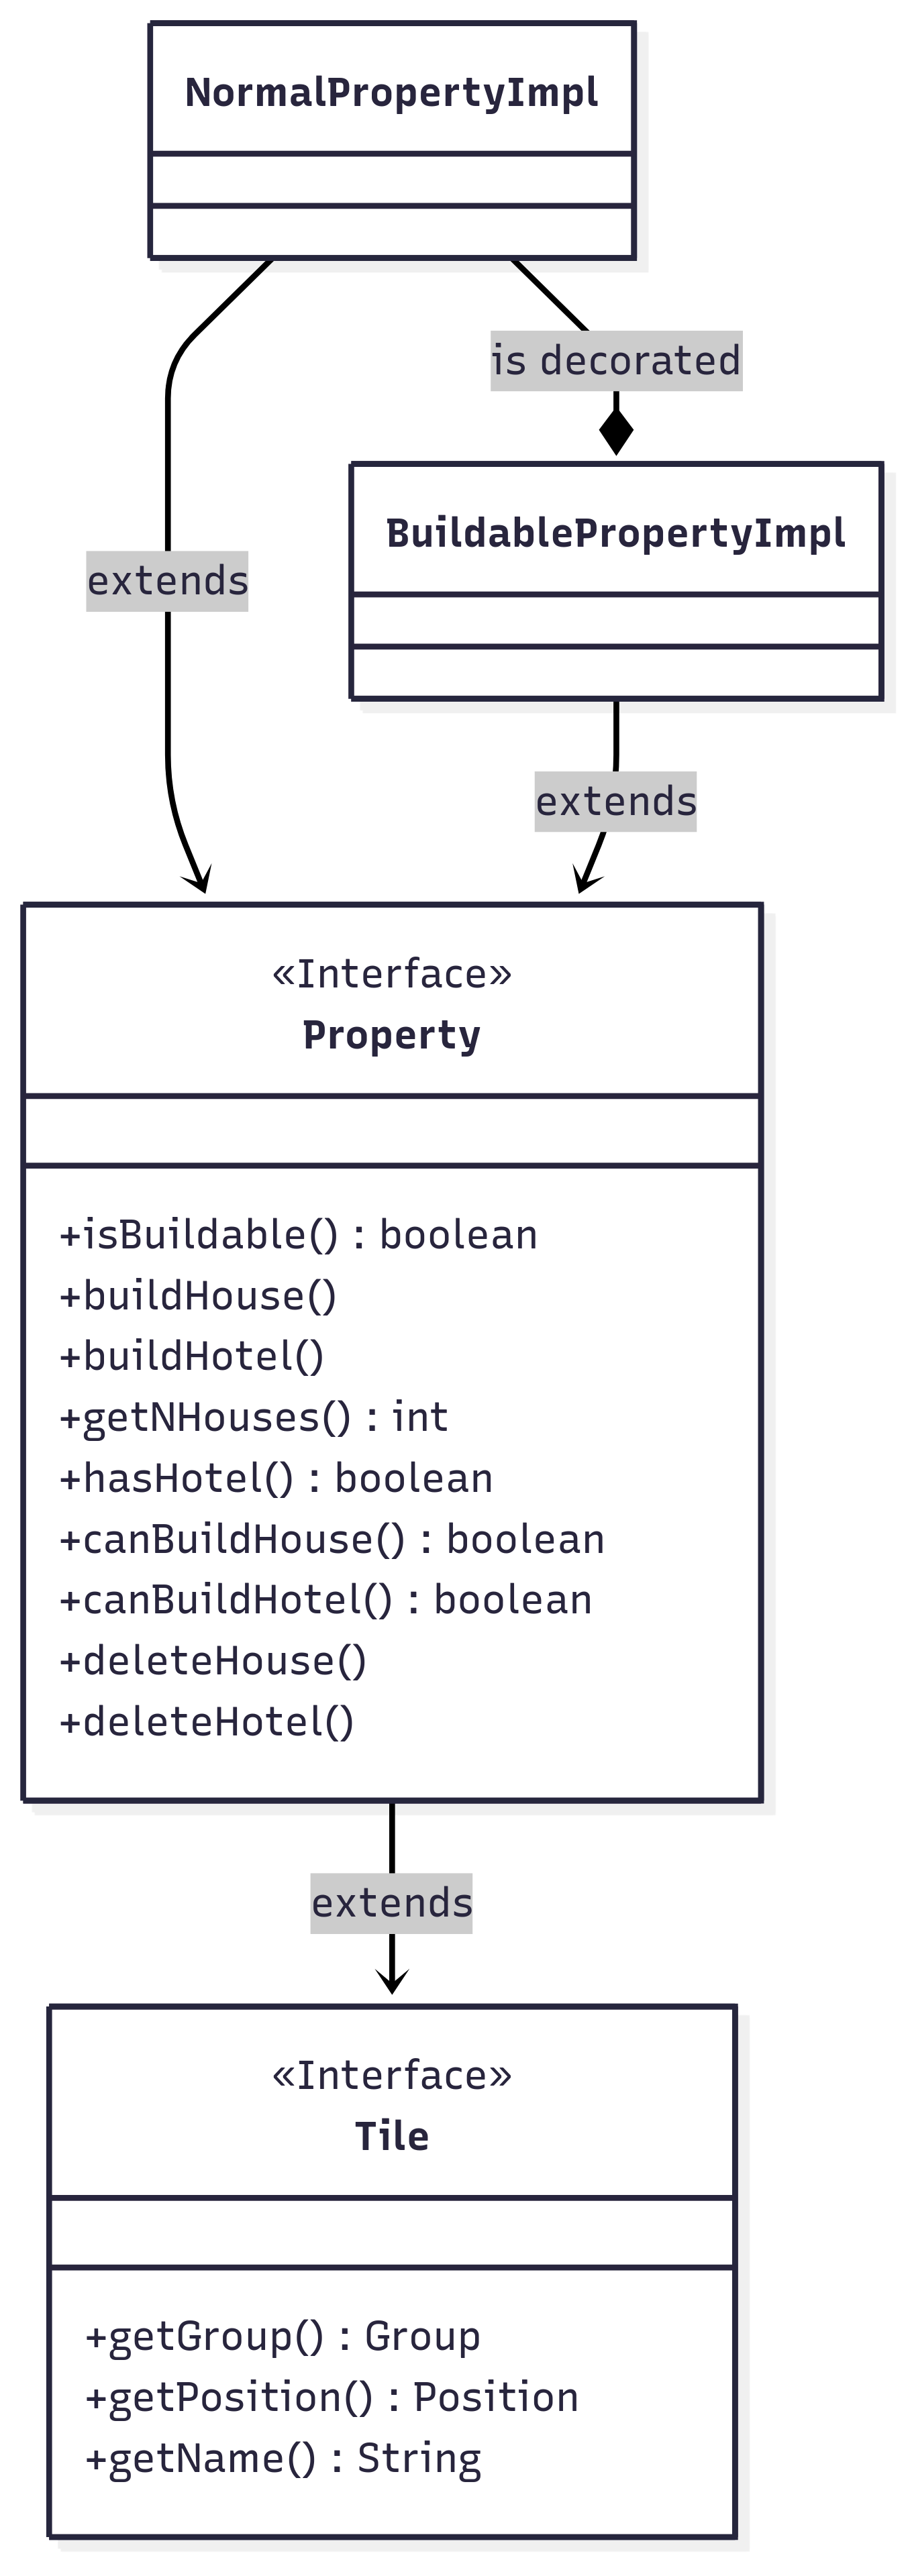
\includegraphics[width=0.5\textwidth]{img/minniti/buildable.png}}	
    \caption{Schema UML che definisce la struttura delle tile e più nello specifico delle property, 
    le property normali sono quelle che non posso costruire appalti mentre le buildable property sono i decorator che contengono all'interno le proprietà normali e gestiscono
    la creazione e rimozione di case e alberghi}
	\label{img:Property}
\end{figure}
Le \textbf{Tiles} si suddividono in \textbf{Property} e \textbf{Special}, queste due tipologie di Tile sono state rappresentate creandole come figlie di Tile,
io mi sono occupato della gestione delle proprietà.\newline

PROBLEMA:
Le proprietà si dividono in proprietà normali in cui si possono costruire case e hotel e proprietà come stazioni e società che non prevedono tale azione. 
Tuttavia tutte le altre azioni si possono svolgere in entrambe di esse e quindi risulta che la proprietà con le case e alberghi diventa una proprietà normale con più opzioni, 
perciò differenziarle in due classi distinte non risultava la scelta ottimale.\newline

SOLUZIONE:
Per risolvere questo problema quindi ho scelto di utilizzare il pattern \textbf{decorator}, in cui si va a creare una proprietà normale (\textbf{NormalPropertyImpl}) 
che non può avere case e hotel e un decoratore chiamato \textbf{BuildablePropertyImpl} che decora la proprietà con le case e gli alberghi,
andando quindi a definire le funzionalità in più che non possono svolgere le stazioni e le società.\newline

\begin{figure}[H]
    \centering
    \makebox[0.5\textwidth]{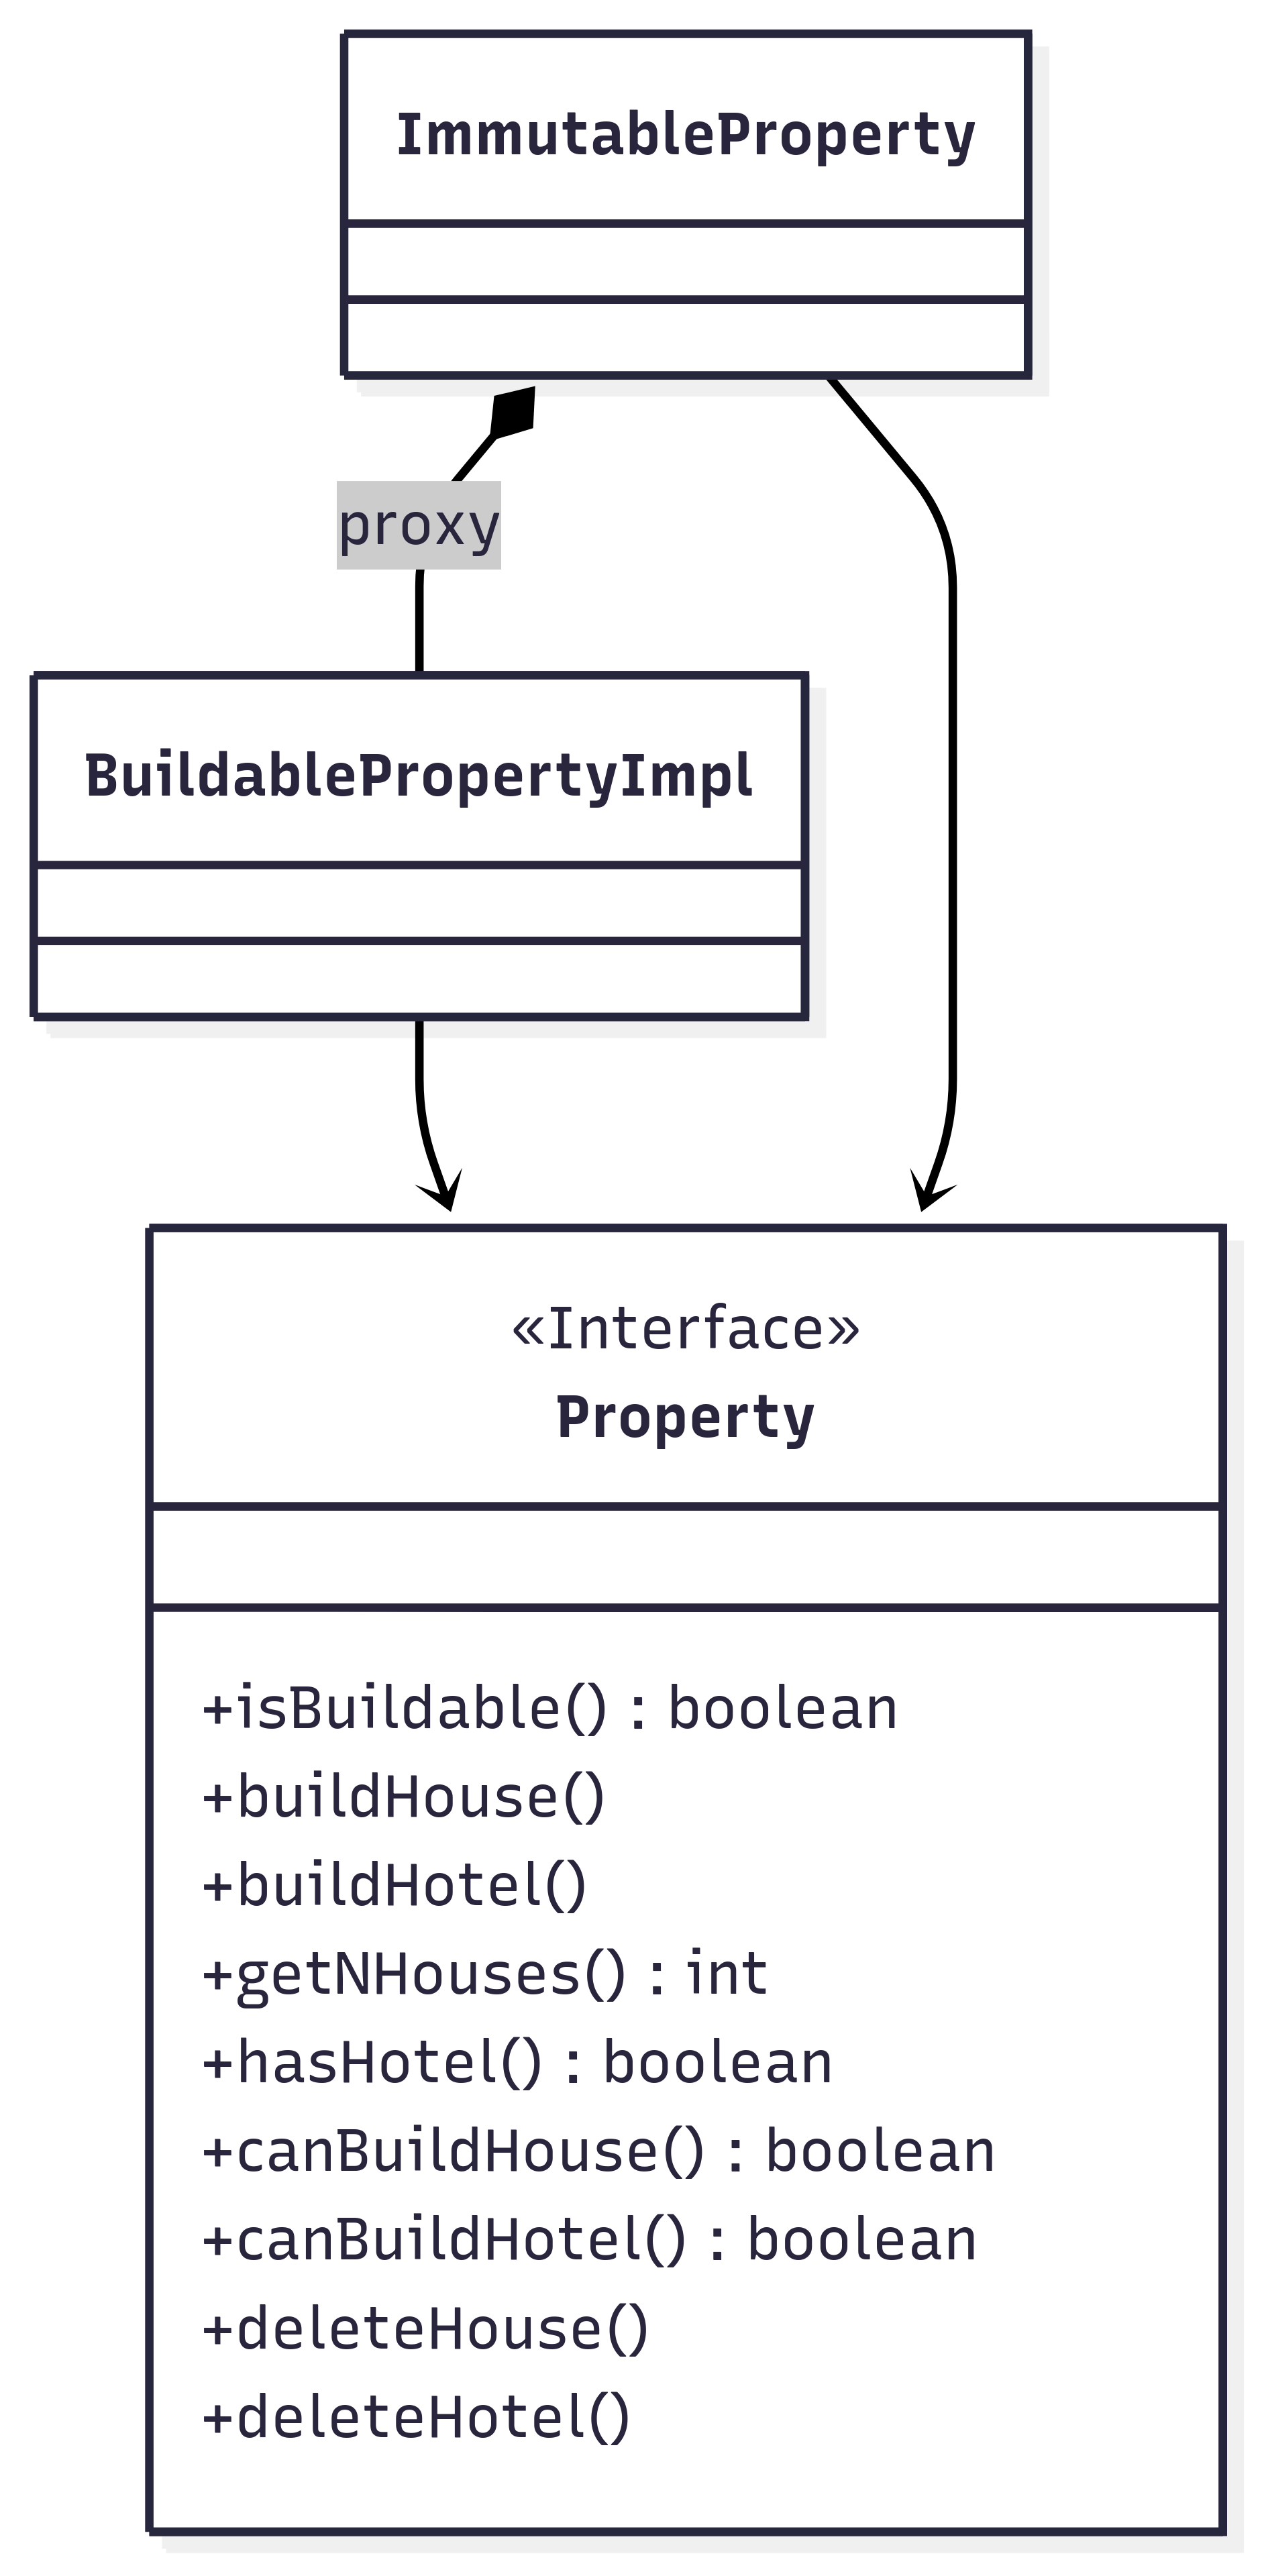
\includegraphics[width=0.5\textwidth]{img/minniti/proxy.png}}	
    \caption{Schema UML che definisce la struttura delle immutable property, 
    le immutable property incapsulano le proprietà edificabili per far ritornare solo le informazioni necessarie al contratto}
	\label{img:Proxy}
\end{figure}
PROBLEMA:
Tutte le proprietà hanno il prezzo dell'affitto che bisogna pagare quando ci passa sopra un giocatore che non è owner, 
tuttavia per le proprietà che possono avere degli appalti tale prezzo cambia in base a quante case sono presenti e se è presente l'hotel.
Quindi la banca dovrà possedere tali informazioni relative alla proprietà ma senza entrare in possesso di altri dati non di sua pertinenza.
Per farlo quindi si potrebbe ricreare sempre un nuovo contratto in cui alla creazione si specifica il nuovo numero di case e la presenza di hotel, 
ma tale soluzione risulterebbe molto poco efficiente.\newline

SOLUZIONE:
Per risolvere questo problema invece ho utilizzato il pattern \textbf{proxy}, 
andando a creare una copia immutabile della proprietà definita come \textbf{ImmutableProperty}, 
che incapsula la proprietà e restituisce solo le informazioni necessarie per il title deed, mentre le altre sono inaccessibili.\newline